\documentclass{beamer}

% for adding conditionals
\usepackage{etoolbox}

% for adding note support
\usepackage{pgfpages}
% only compile notes if `\def\notes{}` in preamble
\ifdef{\notes}{\setbeameroption{show notes on second screen}}{}

\usetheme{CambridgeUS}
\usecolortheme{dolphin}
\usefonttheme{serif}

\definecolor{rit@orange}{HTML}{F36E21}
\definecolor{rit@brown}{HTML}{513127}
\setbeamercolor{structure}{fg=rit@orange}
\setbeamercolor{palette primary}{fg=white, bg=rit@brown}
\setbeamercolor{palette secondary}{fg=rit@brown}
\setbeamercolor{palette tertiary}{fg=white, bg=rit@orange}
\setbeamercolor{titlelike}{fg=rit@brown}
\setbeamercolor{normal text}{fg=rit@brown}

\setbeamertemplate{enumerate}[circle]
\setbeamertemplate{items}[circle]

\AtBeginSection{\frame{\sectionpage}}

\setbeamertemplate{section page}
{
    \begin{centering}
    \begin{beamercolorbox}[sep=12pt,center]{part title}
    \usebeamerfont{section title}\insertsection\par
    \end{beamercolorbox}
    \end{centering}
}

% remove shadow behind blocks
\setbeamertemplate{blocks}[rounded][shadow=false]
% set blocks to use custom color scheme
\setbeamercolor{block title}{bg=rit@orange,fg=white}
\setbeamercolor{block body}{bg=black!5,fg=rit@brown}
% remove shading between block title and body
\makeatletter
\pgfdeclareverticalshading[lower.bg,upper.bg]{bmb@transition}{200cm}{%
  color(0pt)=(lower.bg); color(4pt)=(lower.bg); color(4pt)=(upper.bg)}
\makeatother

\setbeamercovered{dynamic}

\beamertemplatenavigationsymbolsempty

\logo{\vspace{-0.25cm}\includegraphics[width=0.25in]{img/astlogo}}

\pdfpageattr {/Group << /S /Transparency /I true /CS /DeviceRGB>>}

\usepackage{amsmath,amssymb,commath,physics,siunitx,tensor}
\usepackage{aas_macros}
\usepackage{cclicenses,copyrightbox}
\usepackage{float,subcaption}


\usepackage[style=trad-plain,citestyle=authoryear,maxcitenames=3]{biblatex}
\addbibresource{bibliography.bib}


\DeclareCiteCommand{\citefirst}
  {\usebibmacro{prenote}}
  {\renewbibmacro*{name:andothers}{}%
   \usebibmacro{citeindex}%
   \usebibmacro{cite}}
  {\multicitedelim}
  {\usebibmacro{postnote}}

\let\svthefootnote\thefootnote
\textheight 1in
\newcommand\blankfootnote[1]{%
  \let\thefootnote\relax\footnotetext{#1}%
  \let\thefootnote\svthefootnote%
}



\title[Spherical stars]{
  Spherical solutions for stars
}

\author{Daniel Wysocki}

\institute[RIT]{
  Rochester Institute of Technology
}


\date[December 14th, 2015]{
  General Relativity I Presentations
  \\
  December 14th, 2015
}


\begin{document}

\maketitle

\begin{frame}{Introduction}

\begin{itemize}
\setlength\itemsep{24pt}
\item model stars using spherical symmetry
\item Schwarzschild metric
\item T--O--V equation
\item applications
\end{itemize}


\note{

  \begin{itemize}
  \item I will model stars using GR assuming spherical symmetry
  \item I will derive the Schwarzschild metric and T--O--V equation
  \item finally I will relate these equations to modeling specific types of stars
  \end{itemize}

}

\end{frame}

%%%%%%%%



\section{Spherically symmetric coordinates}

\note{

  \begin{itemize}
  \item First we need to derive our coordinate system
  \end{itemize}

}

\begin{frame}{Two-sphere in flat spacetime}

\begin{block}<+->{General metric}
  \begin{displaymath}
    \dd{s}^2 =
   -\dd{t}^2 +
    \dd{r}^2 +
    r^2 (\dd\theta^2 + \sin^2\theta \dd\phi^2)
  \end{displaymath}
\end{block}

\begin{block}<+->{Metric on 2-sphere}
  \begin{displaymath}
    \dd{l}^2 =
    r^2 (\dd\theta^2 + \sin^2\theta \dd\phi^2) \equiv
    r^2 \dd\Omega^2
  \end{displaymath}
\end{block}

\blankfootnote{\textcite[p. 256]{Schutz}}


\note{

  \begin{itemize}
  \item we start with the simplest spherically symmetric coordinates
  \item 2-sphere in Minkowski space
  \end{itemize}

}

\end{frame}

%%%%

\begin{frame}{Two-sphere in curved spacetime}

\begin{block}<+->{Metric on 2-sphere}
  \begin{displaymath}
    \dd{l}^2 =
    f(r', t) \dd\Omega^2
  \end{displaymath}
\end{block}

\begin{block}<+->{Relation to $r$}
  \begin{displaymath}
    f(r', t) \equiv r^2
  \end{displaymath}
\end{block}

\blankfootnote{\textcite[pp. 256--257]{Schutz}}


\note{

  \begin{itemize}
  \item generalize to 2-sphere in arbitrary curved spherically symmetric spacetime
  \item inclusion of curvature makes $r^2$ some function of $r'$ and $t$
  \end{itemize}

}

\end{frame}

%%%%

\begin{frame}{Meaning of $r$}

\begin{columns}[c]
  \begin{column}{0.3\textwidth}
    \begin{figure}[ht]
      \centering
      \copyrightbox[r]{
        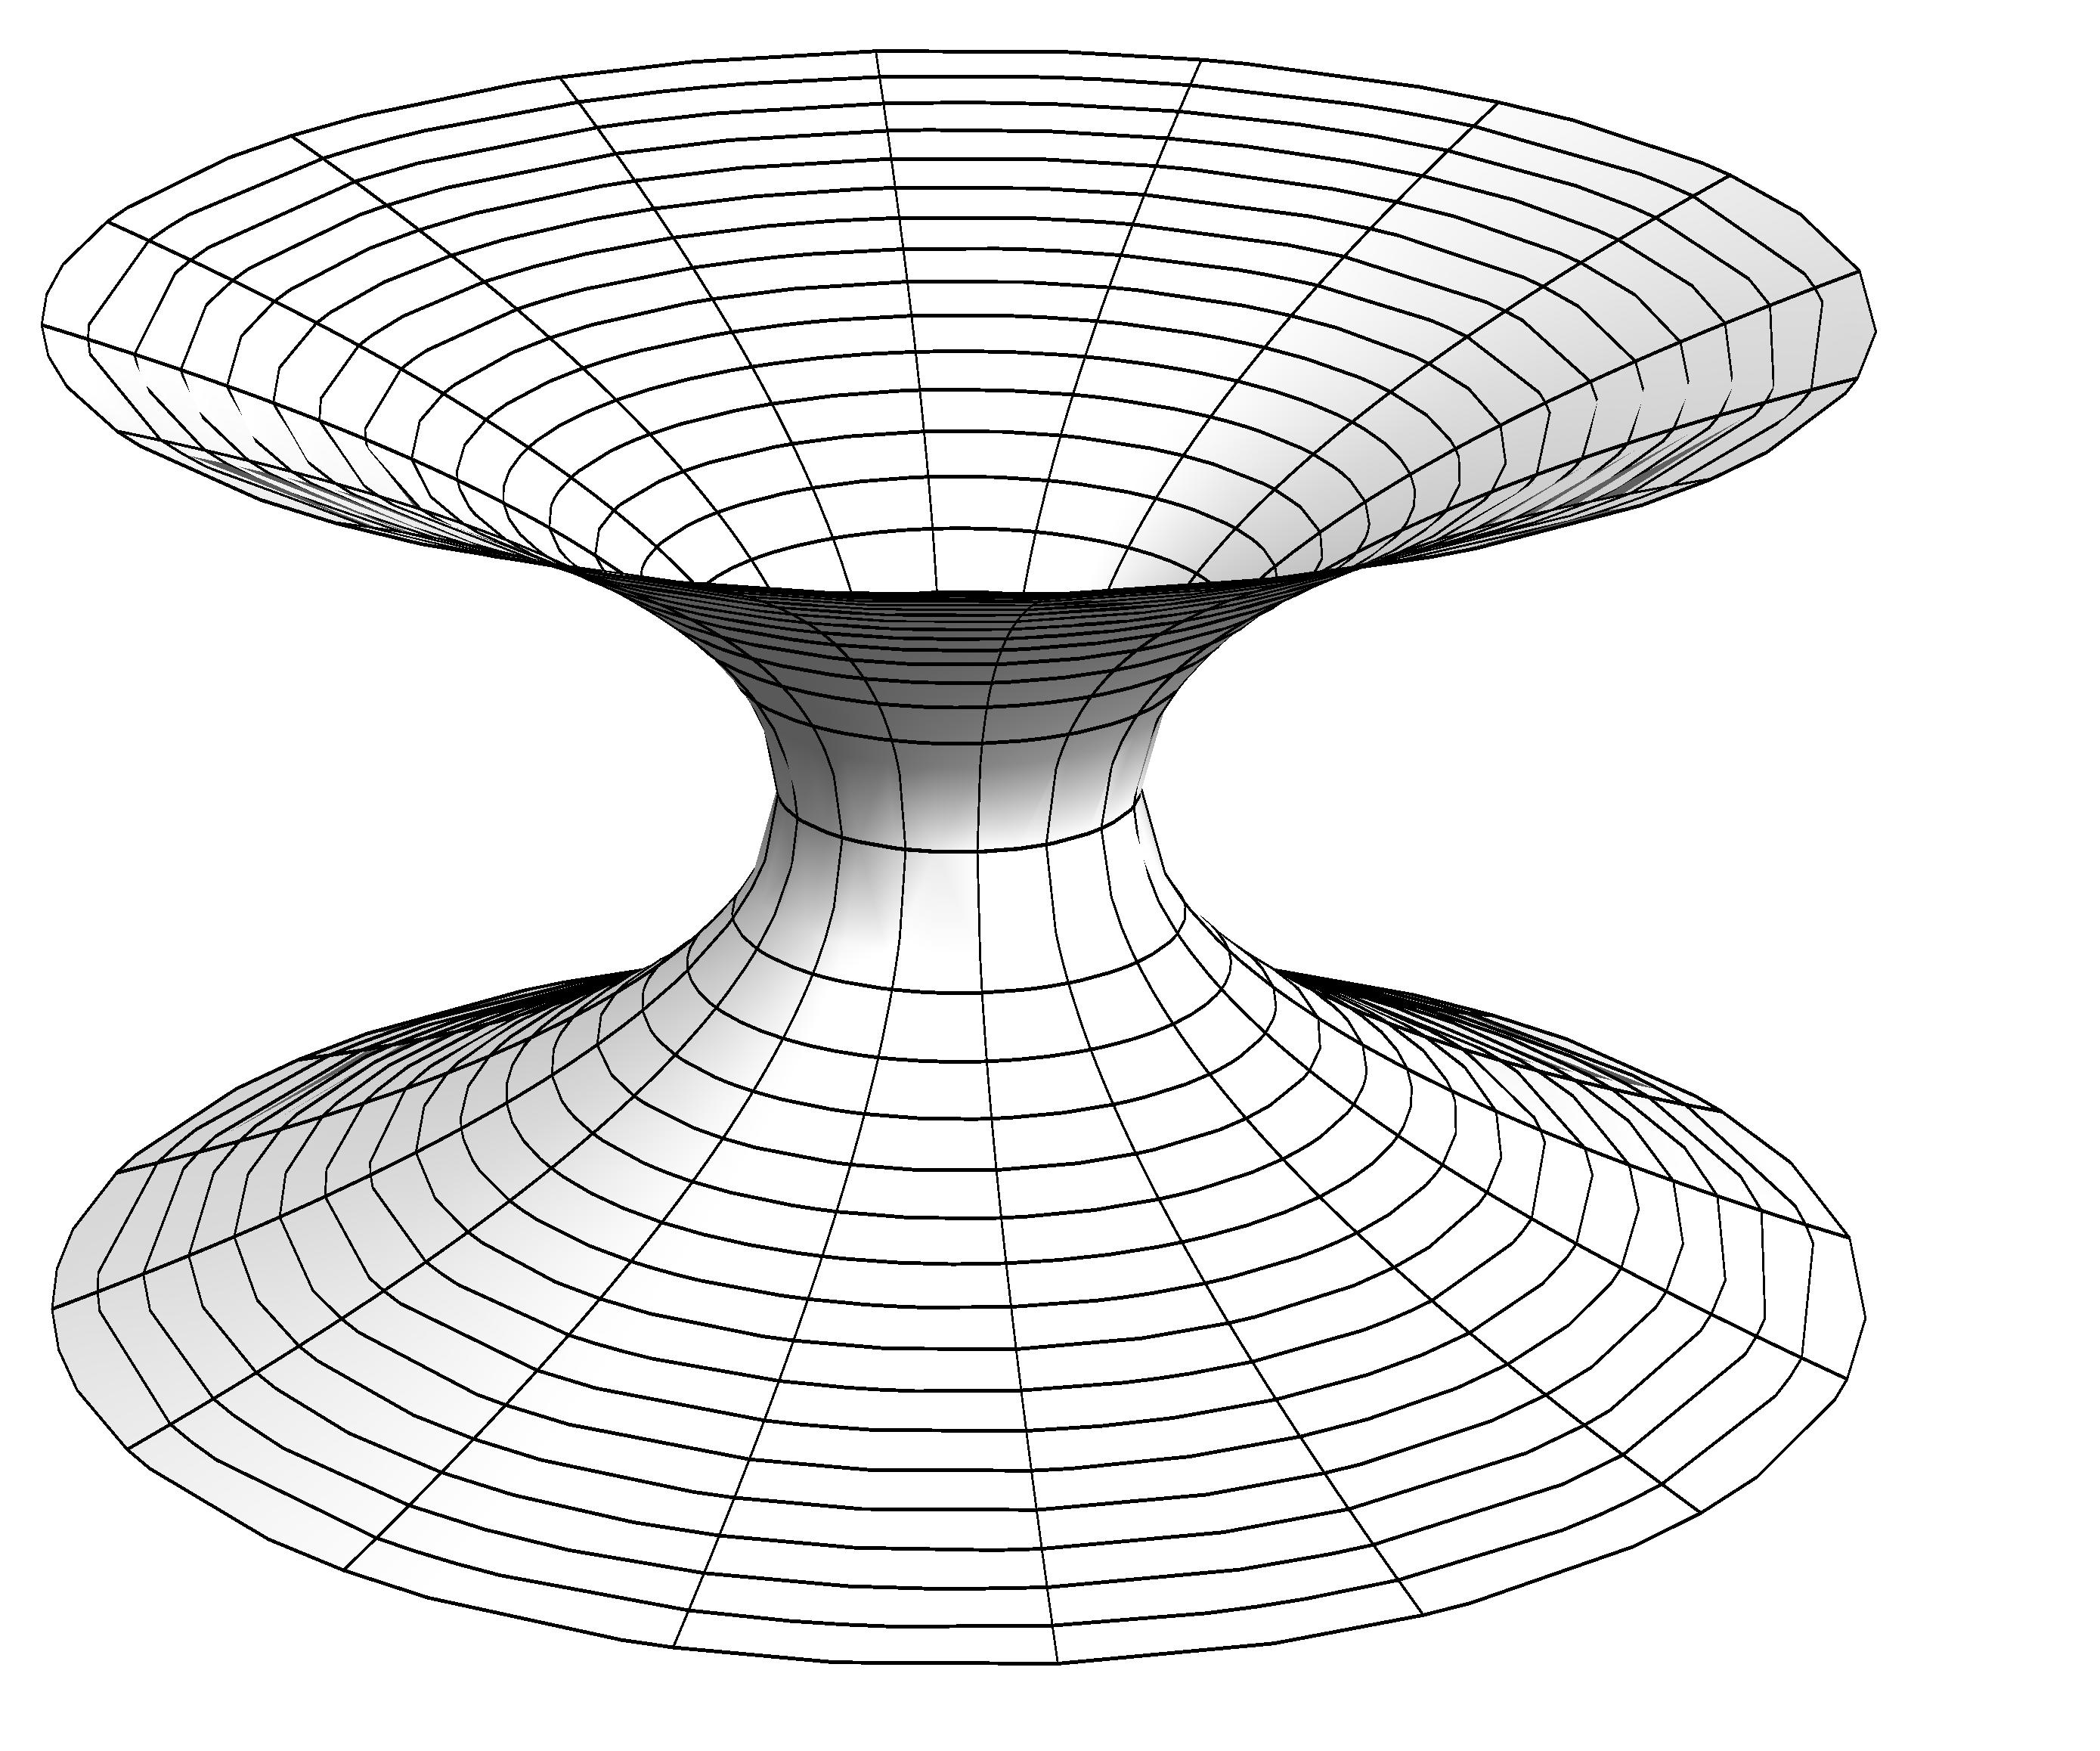
\includegraphics[width=\textwidth]{img/wormhole}
      }{
        Mark Hannam
      }
      \caption{\\Surface with circular symmetry but no coordinate $r = 0$.}
    \end{figure}
  \end{column}

  \begin{column}{0.6\textwidth}
    \begin{itemize}
    \item<+-> \emph{not} proper distance from center
    \item<+-> ``curvature'' or ``area'' coordinate
      \begin{itemize}
      \item radius of curvature and area
      \end{itemize}
    \item<+-> $r =$ const, $t =$ const
      \begin{itemize}
      \item $A = 4 \pi r^2$
      \item $C = 2 \pi r$
      \end{itemize}
    \end{itemize}
  \end{column}
\end{columns}

\blankfootnote{\textcite[p. 257]{Schutz}}


\note{

  \begin{itemize}
  \item $r$ is not necessary the ``distance from the center''
  \item it is merely a coordinate
  \item for instance, we may have a spacetime where the center is missing
    \begin{itemize}
    \item example: wormhole spacetime
    \end{itemize}
  \item surface of constant $(r, t)$ is a two-sphere of area $A$ and
    circumference $C$
  \end{itemize}

}

\end{frame}

%%%%

\begin{frame}{Spherically symmetric spacetime}

\begin{block}{General metric}
  \begin{displaymath}
    \dd{s}^2 =
    g_{00} \dd{t}^2 +
    2 g_{0r} \dd{r} \dd{t} +
    g_{rr} \dd{r}^2 +
    r^2 \dd\Omega^2
  \end{displaymath}
\end{block}

\begin{center}
$g_{00}$, $g_{0r}$, and $g_{rr}$ functions of $t$ and $r$
\end{center}

\blankfootnote{\textcite[p. 258]{Schutz}}


\note{

  \begin{itemize}
  \item now consider not only surface of 2-sphere, but whole spacetime
  \item now we have some unknown $g_{00}$, $g_{rr}$, and cross term $g_{0r}$
  \item cross terms $g_{0i}$ for $i \in \{\theta, \phi\}$ are zero from symmetry
  \item need more constraints to say anything particular about them
  \end{itemize}

}

\end{frame}

%%%%%%%%



\section{Static spacetimes}

\note{

  \begin{itemize}
  \item now I will impose the static constraint
  \end{itemize}

}

\begin{frame}{Motivation}

\begin{itemize}
\setlength\itemsep{24pt}
\item<+-> leads to simple derivation of Schwarzschild metric
\item<+-> unique solution to spherically symmetric, asymptotically
  flat Einstein vacuum field equations (Birkhoff's theorem)
\end{itemize}

\blankfootnote{\textcite[p. 263]{Schutz} and \textcite[p. 843]{MTW}}


\note{

  \begin{itemize}
  \item we choose the contstraint of a static spacetime because
    \begin{itemize}
    \item it allows us to easily derive the Schwarzschild metric
    \item according to Birkhoff's theorem, this metric is the unique
      solution to the Einstein vacuum field equations for spherically
      symmetric, asymptotically flat spacetimes
    \end{itemize}
  \item George David Birkhoff
  \end{itemize}

}

\end{frame}


\begin{frame}{Definition}

A spacetime is static if we can find a time coordinate $t$ for which

\begin{enumerate}[(i)]
\item<+-> the metric independent of $t$

  \begin{displaymath}
    g_{\alpha\beta,t} = 0
  \end{displaymath}

\item<+-> the geometry unchanged by time reversal

  \begin{displaymath}
    t \to -t
  \end{displaymath}

\end{enumerate}

\blankfootnote{\textcite[p. 258]{Schutz}}

\note{

  \begin{itemize}
  \item now I define ``static''
  \item first condition is that the metric is independent of time
    \begin{itemize}
    \item by itself, this condition is called ``stationary''
    \end{itemize}
  \item second condition is that metric unaffected by time reversal
  \item e.g. rotating stars are stationary but not static
  \end{itemize}

}

\end{frame}

%%%%

\begin{frame}{Time reversal}

\onslide<+->{

\begin{displaymath}
  \vb{\Lambda}: (t, x, y, z) \to (-t, x, y, z)
\end{displaymath}

\begin{displaymath}
  g_{\bar\alpha \bar\beta} =
  \tensor{\Lambda}{^\alpha_{\bar\alpha}}
  \tensor{\Lambda}{^\beta_{\bar\beta}}
  g_{\alpha\beta} =
  g_{\alpha\beta}
\end{displaymath}

}

\begin{columns}[t]
  \begin{column}{0.4\textwidth}
    \begin{block}<+->{Transformation}
      \begin{align*}
        \tensor{\Lambda}{^0_{\bar0}} &=
        \tensor{x}{^0_{,\bar0}} = -\tensor{x}{^0_{,0}} = -1
        \\
        \tensor{\Lambda}{^i_{\bar{i}}} &=
        \tensor{x}{^i_{,\bar{i}}} = \tensor{x}{^i_{,i}} = 1
      \end{align*}
    \end{block}
  \end{column}

  \begin{column}{0.4\textwidth}
    \begin{block}<+->{Metric}
      \begin{align*}
        g_{\bar0 \bar0} &=
        (\tensor{\Lambda}{^0_{\bar0}})^2 g_{00} =
        g_{00}
        \\
        g_{\bar{r} \bar{r}} &=
        (\tensor{\Lambda}{^r_{\bar{r}}})^2 g_{rr} =
        g_{rr}
        \\
        g_{\bar0 \bar{r}} &=
        \tensor{\Lambda}{^0_{\bar0}} \tensor{\Lambda}{^r_{\bar{r}}} g_{0r} =
        -g_{0r}
      \end{align*}
    \end{block}
  \end{column}
\end{columns}

\blankfootnote{\textcite[p. 258]{Schutz}}


\note{

  \begin{itemize}
  \item now I use the static constraint to simplify the metric
  \item transformation
    \begin{itemize}
    \item $(0,0)$ term is $\dv*{t}{(-t)}$
    \item spatial terms are $1$ if transformed to themselves
    \item cross-terms are all zero, as coordinates independent of each other
    \end{itemize}
  \item transformed metric
    \begin{itemize}
    \item $(0,0)$ term is unchanged, as $-1$ is squared
    \item $(r,r)$ term is unchanged, as transformation is $1$
    \item $(0,r)$ term is negated, but must still be equal, so it's zero
      \begin{itemize}
      \item no cross terms
      \end{itemize}
    \end{itemize}
  \end{itemize}

}

\end{frame}

%%%%

\begin{frame}{The metric}

\begin{block}<+->{Simplified metric}
\begin{displaymath}
  \dd{s}^2 =
  g_{00} \dd{t}^2 +
  g_{rr} \dd{r}^2 +
  r^2 \dd\Omega^2
\end{displaymath}
\end{block}

\begin{block}<+->{Replacement}
\begin{displaymath}
  g_{00} \to -e^{2\Phi},
  \quad
  g_{rr} \to e^{2\Lambda},
  \quad
  \text{provided $g_{00} < 0 < g_{rr}$}
\end{displaymath}
\end{block}

\begin{block}<+->{Static spherically symmetric metric}
\begin{displaymath}
  \dd{s}^2 =
  -e^{2\Phi} \dd{t}^2 +
  e^{2\Lambda} \dd{r}^2 +
  r^2 \dd\Omega^2
\end{displaymath}
\begin{displaymath}
  \lim_{r\to\infty} \Phi(r) = \lim_{r\to\infty} \Lambda(r) = 0
\end{displaymath}
\end{block}

\blankfootnote{\textcite[pp. 258--259]{Schutz}}


\note{

  \begin{itemize}
  \item now we simplify the metric, since the cross term is zero
  \item we assume $g_{00}$ to be negative, and $g_{rr}$ to be positive
    \begin{itemize}
    \item signature is $(-,+,+,+)$
    \item holds inside stars but not black holes
    \end{itemize}
  \item limits at infinity tell us that spacetime is \emph{asymptotically flat}
    \begin{itemize}
    \item $\Phi = \Lambda = 0 \implies e^{2\Phi} = e^{2\Lambda} = 1$
      and $\vb{g} = \vb{\eta}$
    \end{itemize}
  \end{itemize}

}

\end{frame}

%%%%

\begin{frame}{Einstein Tensor}

\begin{block}<+->{General Einstein tensor}
\begin{displaymath}
  G_{\alpha\beta} = R^{\alpha\beta} - \frac{1}{2} g_{\alpha\beta} R
\end{displaymath}
\end{block}

\begin{block}<+->{Einstein tensor components}
\begin{align*}
  G_{00} &=
  \frac{1}{r^2} e^{2\Phi} \dv{r} [r (1 - e^{-2\Lambda})]
  \\
  G_{rr} &=
  -\frac{1}{r^2} e^{2\Lambda} (1 - e^{-2\Lambda}) + \frac{2}{r} \Phi'
  \\
  G_{\theta\theta} &=
  r^2 e^{-2\Lambda} [\Phi'' + (\Phi')^2 + \Phi' / r - \Phi' \Lambda' - \Lambda' / r]
  \\
  G_{\phi\phi} &=
  \sin^2\theta G_{\theta\theta}
\end{align*}
\end{block}

\blankfootnote{\textcite[pp. 165, 260]{Schutz}}


\note{

  \begin{itemize}
  \item now we can use the metric to derive the Riemann tensor
  \item from that the Einstein tensor
  \item the derivation is involved, so we will just take them as is
  \item we're going to use some of these components later on
  \item $x' \equiv \dv*{x}{r}$
  \end{itemize}

}

\end{frame}

%%%%%%%%



\section{Static perfect fluid}

\note{

  \begin{itemize}
  \item stars are fluids -- for simplicity we assume perfect
  \item thus we will impose additional constraints accordingly
  \end{itemize}

}

\begin{frame}{Four-velocity}

\begin{block}<+->{Constraints}
\begin{align*}
  U^i &= 0
  \text{ (static)}
  &
  \vec{U} \cdot \vec{U} &= -1
  \text{ (conservation law)}
\end{align*}
\end{block}

\begin{block}<+->{Solving for $U^0$}
\begin{displaymath}
  g_{00} U^0 U^0 = -1 \implies
  U^0 = (-g_{00})^{-1/2} = e^{-\Phi}
\end{displaymath}
\end{block}

\begin{block}<+->{Solving for $U_0$}
\begin{displaymath}
  U_0 = g_{00} U^0 = -e^{\Phi}
\end{displaymath}
\end{block}

\blankfootnote{\textcite[p. 260]{Schutz}}


\note{

  \begin{itemize}
  \item static fluid, so in MCRF three-velocity components all zero
  \item we find the only non-zero term, $U^0$, by relating to the dot product
  \item lower it with the metric, to use in next part
  \end{itemize}

  \begin{align*}
    g_{00} U^0 U^0 = -1 \implies
    (U^0)^2 &= (-g_{00})^{-1}
    \\ \implies
    U^0 &= (-g_{00})^{-1/2}
    \\ \implies
    U^0 &= (e^{2\Phi})^{-1/2} = e^{-\Phi}
  \end{align*}

}

\end{frame}

%%

\begin{frame}{Stress--energy tensor}

\begin{block}<+->{Stress-energy tensor for perfect fluid}
\begin{displaymath}
  T_{\alpha\beta} = (\rho + p) U_\alpha U_\beta + p g_{\alpha\beta}
\end{displaymath}
\end{block}

\begin{block}<+->{Components of $T_{\alpha\beta}$}
\begin{align*}
\onslide<.->{
  T_{i\alpha} &= p g_{i\alpha}
}
  \\
\onslide<+->{
  T_{\alpha\beta} & \text{ is diagonal}
}
  \\
\onslide<+->{
  T_{00} &= (\rho + p) e^{2\Phi} + p (-e^{2\Phi}) = \rho e^{2\Phi}
}
  \\
\onslide<+->{
  T_{rr} &= p e^{2\Lambda}
}
\onslide<+->{, \quad
  T_{\theta\theta} = p r^2
}
\onslide<+->{, \quad
  T_{\phi\phi} = p r^2 \sin^2\theta
  \onslide<+->{
    = T_{\theta\theta} \sin^2\theta
  }
}
\end{align*}
\end{block}

\blankfootnote{\textcite[p. 260]{Schutz}}


\note{

  \begin{itemize}
  \item $T_{i\alpha} = p g_{i\alpha}$ because spatial components of $U$ are zero
  \item $T_{\alpha\beta}$ is diagonal because of previous condition
    and $g_{\alpha\beta}$ is diagonal
  \item $T_{00}$ requires a little algebra
  \item $T_{ii}$ just need to multiply metric by $p$
  \item $T_{\phi\phi}$ can be written in terms of $T_{\theta\theta}$
  \end{itemize}

}

\end{frame}

%%%%

\begin{frame}{Equation of state}

\begin{block}{Local thermodynamic equilibrium}
\begin{displaymath}
  p = p(\rho, S) \approx p(\rho)
\end{displaymath}
\end{block}

\begin{itemize}
\item pressure related to energy density and specific entropy
\item we often deal with negligibly small entropies
\end{itemize}

\blankfootnote{\textcite[p. 261]{Schutz}}


\note{

  \begin{itemize}
  \item in a static fluid we have local thermodynamic equilibrium
  \item pressure a function of density and specific entropy
  \item specific entropy assumed negligibly small
  \end{itemize}

}

\end{frame}

%%%

\begin{frame}{Equations of motion}

\begin{block}<+->{Conservation of 4-momentum}
\begin{displaymath}
  \tensor{T}{^{\alpha\beta}_{;\beta}} = 0
\end{displaymath}
\end{block}

\begin{itemize}
\item<+-> symmetries make only non-trivial solution $\alpha = r$

\textbf{TODO: prove}
\end{itemize}

\begin{block}<+->{Equation of motion}
\begin{displaymath}
  (\rho + p) \dv{\Phi}{r} = -\dv{\rho}{r}
\end{displaymath}
\end{block}

\blankfootnote{\textcite[pp. 175, 261]{Schutz}}


\note{

  \begin{itemize}
  \item first equation follows from conservation of 4-momentum
  \item due to symmetry, the only non-trivial solution is for $\alpha = r$
  \item equation of motion for perfect fluid
  \end{itemize}

}

\end{frame}

%%%%

\begin{frame}{Mass function}

\begin{block}<1->{Einstein field equations}
\begin{displaymath}
  {\color<2>{red} G_{00}} = 8 \pi {\color<2>{blue} T_{00}}
\onslide<2->{
  \implies
  {\color<2>{red} \frac{1}{r^2} e^{2\Phi}
                  \dv{r} [{\color<3>{red} r (1 - e^{-2\Lambda})}]} =
  8 \pi {\color<2>{blue} \rho e^{2\Phi}}
}
\end{displaymath}
\end{block}

\begin{block}<3->{$m(r)$}
\begin{displaymath}
  m(r) \equiv {\color<3>{red} \frac{1}{2} r (1 - e^{-2\Lambda})}
  \quad \textrm{or} \quad
  g_{rr} = e^{2\Lambda} \equiv \qty(1 - \frac{2 m(r)}{r})^{-1}
\end{displaymath}
\end{block}

\begin{block}<4->{Relation to energy density}
\begin{displaymath}
  \dv{m(r)}{r} = 4 \pi r^2 \rho
\end{displaymath}
\end{block}

\blankfootnote{\textcite[pp. 260--262]{Schutz}}


\note{

  \begin{itemize}
  \item inspect $(0,0)$ component of Einstein equations
  \item define the mass function, $m(r)$
  \item in Newtonian limit, $m(r)$ is mass within radius $r$

  \begin{displaymath}
    m(r) = 4 \pi \int_0^r (r')^2 \rho(r') \dd{r'}
  \end{displaymath}

  \item doesn't work in GR, because total energy is not localizable
  \end{itemize}

}

\end{frame}

%%%%

\begin{frame}{$\Phi(r)$}

\begin{block}<1->{Einstein field equations}
\begin{displaymath}
  {\color<2>{red} G_{rr}} = 8 \pi {\color<2>{blue} T_{rr}}
\onslide<2->{
  \implies
  {\color<2>{red}
     -\frac{1}{r^2} e^{2\Lambda} (1 - e^{-2\Lambda}) + \frac{2}{r} \Phi'
  } =
  8 \pi {\color<2>{blue} p e^{2\Lambda}}
}
\end{displaymath}
\end{block}

\begin{block}<3->{$\Phi(r)$}
\begin{displaymath}
  \dv{\Phi(r)}{r} = \frac{m(r) + 4 \pi r^3 p}{r [r - 2 m(r)]}
\end{displaymath}
\end{block}

\blankfootnote{\textcite[pp. 260--262]{Schutz}}


\note{

  \begin{itemize}
  \item inspect $(r,r)$ component of Einstein equations
  \item gives us an expression for $\Phi(r)$
  \end{itemize}

}

\end{frame}



%%%%%%%%

\section{Exterior Geometry}

\note{

  \begin{itemize}
  \item until now, we've not considered whether we were inside or outside star
  \item properties inside different than outside (obviously)
  \item we're going to inspect both cases, starting with outside
  \end{itemize}

}

\begin{frame}{Schwarzschild metric I}

\begin{block}<+->{Condition}
\begin{displaymath}
  \rho = p = 0
\end{displaymath}
\end{block}

\begin{block}<+->{Consequences}
\begin{align*}
\onslide<.->{
  \dv{m(r)}{r} &=
  4 \pi r^2 \rho = 0
}
  &
\onslide<+->{
  m(r) &\equiv M
}
  \\
\onslide<+->{
  \dv{\Phi(r)}{r} &=
  \frac{m(r) + 4 \pi r^3 p}{r [r - 2 m(r)]} = \frac{M}{r (r - 2 M)}
}
  &
\onslide<+->{
  \Phi(r) &=
  \frac{1}{2} \log(1 - \frac{2 M}{r})
}
\end{align*}
\end{block}

\blankfootnote{\textcite[pp. 262--263]{Schutz}}


\note{

  \begin{itemize}
  \item the external conditions just state we are in a vaccuum
    \begin{itemize}
    \item breaks down when matter surrounds star
    \end{itemize}
  \item $m(r)$ is constant, we call it $M$
  \item $\dv*{\Phi}{r}$ simplifies, and we can now integrate it to find $\Phi(r)$
  \end{itemize}

}

\end{frame}

%%%%

\begin{frame}{Schwarzschild metric II}

\begin{block}<+->{First two metric components}
\begin{align*}
\onslide<.->{
  g_{rr} &= e^{2\Lambda} = \qty(1 - \frac{2M}{r})^{-1}
}
  &
\onslide<+->{
  g_{00} &= -e^{2\Phi} = -\qty(1 - \frac{2M}{r})
}
\end{align*}
\end{block}

\begin{block}<+->{Schwarzschild metric}
\begin{displaymath}
  \dd{s}^2 =
 -\qty(1 - \frac{2M}{r}) \dd{t}^2 +
  \qty(1 - \frac{2M}{r})^{-1} \dd{r}^2 +
  r^2 \dd{\Omega}^2
\end{displaymath}
\end{block}

\blankfootnote{\textcite[pp. 258, 262--263]{Schutz}}


\note{

  \begin{itemize}
  \item recall $g_{rr}$ from earlier
  \item substituting our expression from $\Phi(r)$ into $-e^{2\Phi}$ gives $g_{00}$
  \item we have found the Schwarzschild metric!
  \end{itemize}

}

\end{frame}

%%%%

\begin{frame}{Far-field metric}

\begin{block}<1->{Condition}
\begin{displaymath}
  r \gg M
\end{displaymath}
\end{block}

\begin{block}<2->{\onslide<3->{Far-field} Schwarzschild metric}
\begin{displaymath}
  \dd{s}^2 \only<-2>{{=}} \only<3->{{\approx}}
 -\qty(1 - \frac{2M}{r}) \dd{t}^2 +
  \qty(1 \only<-2>{-} \only<3->{+} \frac{2M}{r})^{\only<-2>{-1}\only<3->{\phantom{-1}}} \dd{r}^2 +
  r^2 \dd{\Omega}^2
\end{displaymath}
\end{block}

\begin{block}<4->{Far-field Schwarzschild metric (Cartesian)}
\begin{displaymath}
  \dd{s}^2 \approx
 -\qty(1 - \frac{2M}{R}) \dd{t}^2 +
  \qty(1 + \frac{2M}{R}) (\dd{x}^2 + \dd{y}^2 + \dd{z}^2)
\end{displaymath}
\end{block}

\onslide<4->{
\begin{displaymath}
  R^2 \equiv x^2 + y^2 + z^2
\end{displaymath}
}

\blankfootnote{\textcite[pp. 263]{Schutz}}


\note{

  \begin{itemize}
  \item far-field metric of a star (far away)
    \begin{itemize}
    \item mass $M$
    \item distance $R$
    \end{itemize}
  \end{itemize}

}

\end{frame}

%%%%

\begin{frame}{Birkhoff's Theorem}

\onslide<+-> {

If the geometry of a given region of spacetime is:

}

\begin{enumerate}
\item<+-> spherically symmetric
\item<+-> a solution to the Einstein field equations in vacuum
\end{enumerate}

\onslide<+->{

then that geometry is necessarily a subset of the Schwarzschild geometry.

}

\vspace{0.5in}

\onslide<+->{

(Proof given in \textcite[pp. 843--844]{MTW})

}

\blankfootnote{\textcite{1923rmp..book.....B}}


\note{

  \begin{itemize}
  \item the Schwarzschild metric generalizes to all spherically
    symmetric spacetimes in a vacuum
  \item George David Birkhoff
  \end{itemize}

}

\end{frame}

%%%%%%%%



\section{Interior structure}

\note{

  \begin{itemize}
  \item now we look at the remaining, and most interesting regime
    \begin{itemize}
    \item inside the star
    \end{itemize}
  \item our assumptions from outside the star no longer hold
  \end{itemize}

}

\begin{frame}{Tolman--Oppenheimer--Volkov (T--O--V) equation}

\begin{block}<+->{Condition}
\begin{displaymath}
  \rho \neq 0 \quad p \neq 0
\end{displaymath}
\end{block}

\begin{block}<+->{Recall}

\begin{columns}[c]
\begin{column}{0.5\textwidth}
\begin{displaymath}
  (\rho + p) \dv{\Phi}{r} = -\dv{p}{r}
\end{displaymath}
\end{column}

\begin{column}<+->{0.5\textwidth}
\begin{displaymath}
  \dv{\Phi}{r} = \frac{m(r) + 4 \pi r^3 p}{r [r - 2 m(r)]}
\end{displaymath}
\end{column}
\end{columns}

\end{block}

\begin{block}<+->{T--O--V equation}
\begin{displaymath}
  \dv{p}{r} =
 -\frac{(\rho + p) [m(r) + 4 \pi r^3 p]}{r [r - 2m(r)]}
\end{displaymath}
\end{block}

\blankfootnote{\textcite[pp. 261--264]{Schutz}}


\note{

  \begin{itemize}
  \item inside a star, we cannot assume density and pressure are zero
  \item revisit two earlier equations
  \item substitute one into the other
  \item arrive at the T--O--V equation
  \end{itemize}

}

\end{frame}

%%%%

\begin{frame}{System of coupled differential equations}

\begin{block}{T--O--V equation}
\begin{displaymath}
  \dv{p}{r} =
 -\frac{(\rho + p) [m(r) + 4 \pi r^3 p]}{r [r - 2m(r)]}
\end{displaymath}
\end{block}

\begin{block}{Mass function}
\begin{displaymath}
  \dv{m(r)}{r} = 4 \pi r^2 \rho
\end{displaymath}
\end{block}

\begin{block}{Equation of state}
\begin{displaymath}
  p = p(\rho)
\end{displaymath}
\end{block}

\blankfootnote{\textcite[pp. 261--262, 264]{Schutz}}


\note{

  \begin{itemize}
  \item T--O--V equation coupled with $\dv*{m}{r}$ and $p(\rho)$
    \begin{itemize}
    \item 3 equations
    \item 3 unknowns ($m$, $\rho$, $p$)
    \item $\Phi(r)$ only intermediate variable
    \end{itemize}
  \item can integrate to find $m(r)$, $\rho(r)$, and $p(r)$
  \end{itemize}

}

\end{frame}


%%%%

\begin{frame}{Newtonian hydrostatic equilibrium}

\begin{block}<+->{Newtonian limit}
\begin{displaymath}
  p \ll \rho;
  \quad
  4 \pi r^3 p \ll m;
  \quad
  m \ll r
\end{displaymath}
\end{block}

\begin{block}<+->{Equation of hydrostatic equilibrium}
\begin{displaymath}
  \dv{p}{r} =
 -\frac{(\rho + {\color{red} p}) [m(r) + {\color{red} 4 \pi r^3 p}]}
       {r [r - {\color{red} 2m(r)}]} =
 -\frac{\rho m(r)}{r^2}
\end{displaymath}
\end{block}

\blankfootnote{\textcite[pp. 265--266]{Schutz} and
               \textcite[p. 3]{1994sipp.book.....H}}


\note{

  \begin{itemize}
  \item in the Newtonian limit we get these constraints
  \item which allow us to cancel terms in the T--O--V equation
  \item and arrive at the familiar equation of HSE
  \end{itemize}

}

\end{frame}


\section{References}

\begin{frame}[allowframebreaks]

\nocite{*}
\printbibliography[heading=subbibliography]

\end{frame}

\end{document}
